% Chapter 10: Comprehensive Review - Complete Time Series Analysis
% Applying all methods to real data: Bitcoin, Sunspots, Unemployment
% Bachelor program, Bucharest University of Economic Studies

\documentclass[9pt, aspectratio=169, t]{beamer}

% Ensure content fits on slides
\setbeamersize{text margin left=8mm, text margin right=8mm}

%=============================================================================
% THEME AND STYLE CONFIGURATION
%=============================================================================
\usetheme{Madrid}
\usecolortheme{seahorse}

% IDA-Inspired Color Palette
\definecolor{MainBlue}{RGB}{26, 58, 110}
\definecolor{AccentBlue}{RGB}{42, 82, 140}
\definecolor{IDAred}{RGB}{220, 53, 69}
\definecolor{DarkGray}{RGB}{51, 51, 51}
\definecolor{MediumGray}{RGB}{128, 128, 128}
\definecolor{LightGray}{RGB}{248, 248, 248}
\definecolor{VeryLightGray}{RGB}{235, 235, 235}
\definecolor{Crimson}{RGB}{220, 53, 69}
\definecolor{Forest}{RGB}{46, 125, 50}
\definecolor{Amber}{RGB}{181, 133, 63}
\definecolor{Orange}{RGB}{230, 126, 34}
\definecolor{BitcoinOrange}{RGB}{247, 147, 26}

\setbeamercolor{palette primary}{bg=MainBlue, fg=white}
\setbeamercolor{palette secondary}{bg=MainBlue!85, fg=white}
\setbeamercolor{palette tertiary}{bg=MainBlue!70, fg=white}
\setbeamercolor{structure}{fg=MainBlue}
\setbeamercolor{title}{fg=MainBlue}
\setbeamercolor{frametitle}{fg=MainBlue, bg=white}
\setbeamercolor{block title}{bg=MainBlue, fg=white}
\setbeamercolor{block body}{bg=VeryLightGray, fg=DarkGray}
\setbeamercolor{block title alerted}{bg=Crimson, fg=white}
\setbeamercolor{block body alerted}{bg=Crimson!8, fg=DarkGray}
\setbeamercolor{block title example}{bg=Forest, fg=white}
\setbeamercolor{block body example}{bg=Forest!8, fg=DarkGray}
\setbeamercolor{item}{fg=MainBlue}

\setbeamertemplate{navigation symbols}{}

\setbeamertemplate{footline}{
    \leavevmode%
    \hbox{%
        \begin{beamercolorbox}[wd=.333333\paperwidth,ht=2.5ex,dp=1ex,center]{author in head/foot}%
            \usebeamerfont{author in head/foot}\insertshortauthor
        \end{beamercolorbox}%
        \begin{beamercolorbox}[wd=.333333\paperwidth,ht=2.5ex,dp=1ex,center]{title in head/foot}%
            \usebeamerfont{title in head/foot}\insertshorttitle
        \end{beamercolorbox}%
        \begin{beamercolorbox}[wd=.333333\paperwidth,ht=2.5ex,dp=1ex,right]{date in head/foot}%
            \usebeamerfont{date in head/foot}\insertshortdate{}\hspace*{2em}
            \insertframenumber{} / \inserttotalframenumber\hspace*{2ex}
        \end{beamercolorbox}}%
    \vskip0pt%
}

%=============================================================================
% PACKAGES
%=============================================================================
\usepackage[utf8]{inputenc}
\usepackage[T1]{fontenc}
\usepackage{amsmath, amssymb, amsthm}
\usepackage{mathtools}
\usepackage{bm}
\usepackage{tikz}
\usetikzlibrary{arrows.meta, positioning, shapes, calc}
\usepackage{booktabs}
\usepackage{multirow}
\usepackage{array}
\usepackage{graphicx}
\usepackage{hyperref}
\hypersetup{colorlinks=false, pdfborder={0 0 0}}
\graphicspath{{../logos/}{../charts/}}

%=============================================================================
% THEOREM ENVIRONMENTS
%=============================================================================
\theoremstyle{definition}
\setbeamertemplate{theorems}[numbered]
\newtheorem{defn}{Definition}
\newtheorem{thm}{Theorem}
\newtheorem{prop}{Proposition}

%=============================================================================
% CUSTOM COMMANDS
%=============================================================================
\newcommand{\E}{\mathbb{E}}
\newcommand{\Var}{\text{Var}}
\newcommand{\Cov}{\text{Cov}}
\newcommand{\Corr}{\text{Corr}}
\newcommand{\R}{\mathbb{R}}

%=============================================================================
% TITLE INFORMATION
%=============================================================================
\title[Chapter 10: Comprehensive Review]{Chapter 10: Comprehensive Review}
\subtitle{Bachelor Program, Faculty of Cybernetics, Statistics and Economic Informatics, Bucharest University of Economic Studies}
\author[Prof. Daniel Traian Pele, PhD]{Prof. Daniel Traian Pele, PhD\\[0.2cm]\footnotesize\texttt{danpele@ase.ro}}
\institute{Bucharest University of Economic Studies}
\date{Academic Year 2025--2026}

\begin{document}

%=============================================================================
% TITLE SLIDE
%=============================================================================
\begin{frame}[plain]
    \begin{tikzpicture}[remember picture, overlay]
        \fill[IDAred] (current page.north west) rectangle ([yshift=-0.15cm]current page.north east);
        \node[anchor=north west] at ([xshift=0.5cm, yshift=-0.3cm]current page.north west) {
            \href{https://www.ase.ro}{\includegraphics[height=1.1cm]{ase_logo.png}}
        };
        \node[anchor=north] at ([yshift=-0.3cm]current page.north) {
            \href{https://ai4efin.ase.ro}{\includegraphics[height=1.1cm]{ai4efin_logo.png}}
        };
        \node[anchor=north east] at ([xshift=-0.5cm, yshift=-0.3cm]current page.north east) {
            \href{https://www.digital-finance-msca.com}{\includegraphics[height=1.1cm]{msca_logo.png}}
        };
    \end{tikzpicture}
    \vfill
    \begin{center}
        {\Large\textcolor{MediumGray}{Time Series Analysis and Forecasting}}\\[0.3cm]
        {\Huge\textbf{\textcolor{MainBlue}{Chapter 10: Comprehensive Review}}}\\[0.5cm]
        {\Large\textcolor{IDAred}{Complete Analysis with Real Data}}
    \end{center}
    \vfill

    \begin{tikzpicture}[remember picture, overlay]
        \fill[IDAred] (current page.south west) rectangle ([yshift=0.15cm]current page.south east);
        \node[anchor=south west] at ([xshift=0.5cm, yshift=0.8cm]current page.south west) {
            \href{https://theida.net}{\includegraphics[height=0.9cm]{ida_logo.png}}
        };
        \node[anchor=south] at ([xshift=-3cm, yshift=0.8cm]current page.south) {
            \href{https://blockchain-research-center.com}{\includegraphics[height=0.9cm]{brc_logo.png}}
        };
        \node[anchor=south] at ([yshift=0.8cm]current page.south) {
            \href{https://quantinar.com}{\includegraphics[height=0.9cm]{qr_logo.png}}
        };
        \node[anchor=south] at ([xshift=3cm, yshift=0.8cm]current page.south) {
            \href{https://quantlet.com}{\includegraphics[height=0.9cm]{ql_logo.png}}
        };
        \node[anchor=south east] at ([xshift=-0.5cm, yshift=0.8cm]current page.south east) {
            \href{https://ipe.ro/new}{\includegraphics[height=0.9cm]{acad_logo.png}}
        };
    \end{tikzpicture}
\end{frame}

%=============================================================================
% TABLE OF CONTENTS
%=============================================================================
\begin{frame}{Outline}
    \tableofcontents
\end{frame}

%=============================================================================
% SECTION 1: INTRODUCTION
%=============================================================================
\section{The Complete Analysis Workflow}

\begin{frame}{Course Overview: Methods Covered}
    \begin{columns}[T]
        \begin{column}{0.48\textwidth}
            \textbf{Classical Methods}
            \begin{itemize}
                \item \textcolor{MainBlue}{Ch 1:} Time Series Fundamentals
                \item \textcolor{MainBlue}{Ch 2:} ARMA Models
                \item \textcolor{MainBlue}{Ch 3:} ARIMA Models
                \item \textcolor{MainBlue}{Ch 4:} SARIMA Models
                \item \textcolor{MainBlue}{Ch 5:} GARCH Models
            \end{itemize}
        \end{column}
        \begin{column}{0.48\textwidth}
            \textbf{Advanced Methods}
            \begin{itemize}
                \item \textcolor{Forest}{Ch 6:} VAR \& Granger Causality
                \item \textcolor{Forest}{Ch 7:} Cointegration \& VECM
                \item \textcolor{Forest}{Ch 8:} Modern Extensions
                \item \textcolor{Forest}{Ch 9:} Prophet \& TBATS
            \end{itemize}
            \vspace{0.5em}
            \textbf{Today: Apply ALL to Real Data!}
        \end{column}
    \end{columns}
\end{frame}

\begin{frame}{The Complete Analysis Workflow}
    \begin{center}
        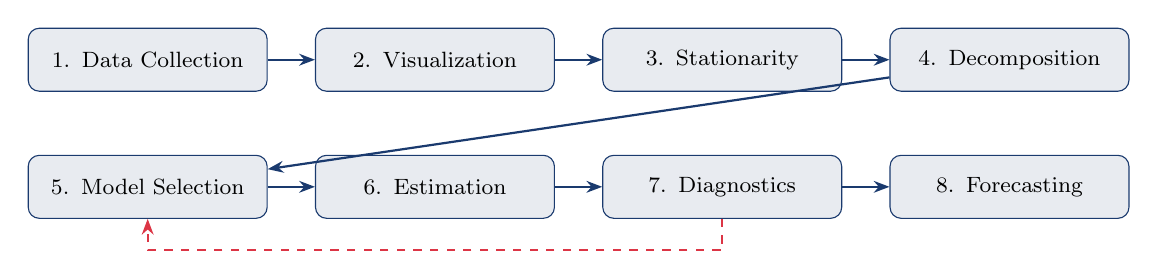
\begin{tikzpicture}[
            node distance=0.6cm,
            box/.style={rectangle, rounded corners, draw=MainBlue, fill=MainBlue!10,
                        text width=2.8cm, minimum height=0.8cm, align=center, font=\footnotesize},
            arrow/.style={-{Stealth[length=2mm]}, thick, MainBlue}
        ]
            % Row 1
            \node[box] (data) {1. Data Collection};
            \node[box, right=of data] (viz) {2. Visualization};
            \node[box, right=of viz] (stat) {3. Stationarity};
            \node[box, right=of stat] (decomp) {4. Decomposition};

            % Row 2
            \node[box, below=0.8cm of data] (model) {5. Model Selection};
            \node[box, right=of model] (est) {6. Estimation};
            \node[box, right=of est] (diag) {7. Diagnostics};
            \node[box, right=of diag] (forecast) {8. Forecasting};

            % Arrows
            \draw[arrow] (data) -- (viz);
            \draw[arrow] (viz) -- (stat);
            \draw[arrow] (stat) -- (decomp);
            \draw[arrow] (decomp) -- (model);
            \draw[arrow] (model) -- (est);
            \draw[arrow] (est) -- (diag);
            \draw[arrow] (diag) -- (forecast);

            % Feedback loop
            \draw[arrow, dashed, IDAred] (diag.south) -- ++(0,-0.4) -| (model.south);
        \end{tikzpicture}
    \end{center}

    \vspace{0.3cm}
    \begin{alertblock}{Key Principle}
        Model diagnostics may require returning to model selection (iterative process)
    \end{alertblock}
\end{frame}

\begin{frame}{Real Datasets for This Chapter}
    \begin{columns}[T]
        \begin{column}{0.24\textwidth}
            \begin{block}{\textcolor{BitcoinOrange}{Bitcoin}}
                \begin{itemize}
                    \item Daily 2019-2024
                    \item Volatility clustering
                    \item ARIMA + GARCH
                \end{itemize}
            \end{block}
        \end{column}
        \begin{column}{0.24\textwidth}
            \begin{block}{\textcolor{Orange}{Sunspots}}
                \begin{itemize}
                    \item Yearly 1900-2023
                    \item 11-year cycle
                    \item Fourier terms
                \end{itemize}
            \end{block}
        \end{column}
        \begin{column}{0.24\textwidth}
            \begin{block}{\textcolor{MainBlue}{Unemployment}}
                \begin{itemize}
                    \item Monthly 2010-2023
                    \item COVID-19 shock
                    \item Prophet
                \end{itemize}
            \end{block}
        \end{column}
        \begin{column}{0.24\textwidth}
            \begin{block}{\textcolor{Forest}{Economic VAR}}
                \begin{itemize}
                    \item Quarterly 2000-2023
                    \item GDP, Inflation, etc.
                    \item Multivariate VAR
                \end{itemize}
            \end{block}
        \end{column}
    \end{columns}
\end{frame}

%=============================================================================
% SECTION 2: CASE STUDY 1 - BITCOIN
%=============================================================================
\section{Case Study 1: Bitcoin Volatility Analysis}

\begin{frame}{Bitcoin: Data Overview}
    \begin{center}
        \includegraphics[width=0.95\textwidth, height=0.70\textheight, keepaspectratio]{ch10_bitcoin_overview.pdf}
    \end{center}

    \begin{itemize}
        \item \textbf{Data:} Bitcoin daily prices and log returns (2019-2024)
        \item \textbf{Key events:} COVID crash, 2021 bull run, crypto winter 2022
    \end{itemize}
\end{frame}

\begin{frame}{Step 1: Stationarity Testing}
    \begin{columns}[T]
        \begin{column}{0.55\textwidth}
            \textbf{Augmented Dickey-Fuller Test}
            \begin{itemize}
                \item $H_0$: Unit root (non-stationary)
                \item $H_1$: Stationary
            \end{itemize}

            \vspace{0.5em}
            \textbf{Results on Bitcoin:}
            \begin{table}[h]
                \footnotesize
                \begin{tabular}{lcc}
                    \toprule
                    Series & ADF Statistic & p-value \\
                    \midrule
                    Prices & $-0.87$ & 0.79 \\
                    Log Returns & $-42.1$ & $<0.001$ \\
                    \bottomrule
                \end{tabular}
            \end{table}

            \vspace{0.5em}
            $\Rightarrow$ Prices: non-stationary (random walk) \\
            $\Rightarrow$ Returns: stationary
        \end{column}
        \begin{column}{0.43\textwidth}
            \begin{exampleblock}{KPSS Test (Confirmation)}
                \begin{itemize}
                    \item $H_0$: Stationary
                    \item $H_1$: Unit root
                \end{itemize}

                \vspace{0.3em}
                Prices: KPSS = 5.83** \\
                Returns: KPSS = 0.12

                \vspace{0.3em}
                \textcolor{Forest}{Both tests confirm: use log returns!}
            \end{exampleblock}
        \end{column}
    \end{columns}
\end{frame}

\begin{frame}{Step 2: ACF/PACF Analysis of Returns}
    \begin{center}
        \includegraphics[width=0.95\textwidth, height=0.65\textheight, keepaspectratio]{ch10_bitcoin_acf_pacf.pdf}
    \end{center}

    \begin{itemize}
        \item \textbf{Returns:} Near white noise (weak linear dependence)
        \item \textbf{Squared returns:} Strong persistence $\Rightarrow$ \textcolor{IDAred}{volatility clustering}
        \item \textbf{Implication:} GARCH model essential for Bitcoin!
    \end{itemize}
\end{frame}

\begin{frame}{Step 3: ARIMA Model for Returns}
    \textbf{Model Selection using AIC/BIC:}

    \begin{columns}[T]
        \begin{column}{0.48\textwidth}
            \begin{table}[h]
                \footnotesize
                \begin{tabular}{lcc}
                    \toprule
                    Model & AIC & BIC \\
                    \midrule
                    ARIMA(0,0,0) & 9524 & 9530 \\
                    ARIMA(1,0,0) & 9522 & 9534 \\
                    ARIMA(0,0,1) & 9523 & 9535 \\
                    \textbf{ARIMA(1,0,1)} & \textbf{9520} & \textbf{9538} \\
                    \bottomrule
                \end{tabular}
            \end{table}

            \vspace{0.3em}
            Best: ARIMA(1,0,1) but marginal improvement
        \end{column}
        \begin{column}{0.48\textwidth}
            \begin{alertblock}{Key Insight}
                Crypto returns are notoriously unpredictable. The ``alpha'' is in understanding \textbf{volatility dynamics}, not predicting direction!
            \end{alertblock}
        \end{column}
    \end{columns}
\end{frame}

\begin{frame}{Step 4: GARCH Model for Volatility}
    \begin{center}
        \includegraphics[width=0.95\textwidth, height=0.60\textheight, keepaspectratio]{ch10_bitcoin_garch.pdf}
    \end{center}

    \textbf{GARCH(1,1) Model:}
    \[
        \sigma_t^2 = \omega + \alpha \varepsilon_{t-1}^2 + \beta \sigma_{t-1}^2
    \]

    \begin{itemize}
        \item Bitcoin shows $\alpha + \beta \approx 0.95$ (high persistence)
        \item COVID and May 2021 periods show massive volatility spikes
    \end{itemize}
\end{frame}

\begin{frame}{Bitcoin: Summary of Approach}
    \begin{center}
        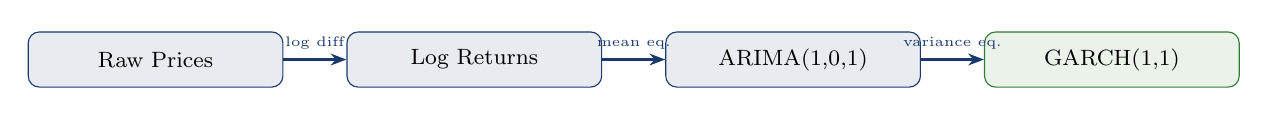
\begin{tikzpicture}[
            node distance=0.4cm,
            box/.style={rectangle, rounded corners, draw=MainBlue, fill=MainBlue!10,
                        text width=3cm, minimum height=0.7cm, align=center, font=\footnotesize},
            result/.style={rectangle, rounded corners, draw=Forest, fill=Forest!10,
                          text width=3cm, minimum height=0.7cm, align=center, font=\footnotesize},
            arrow/.style={-{Stealth[length=2mm]}, thick, MainBlue}
        ]
            \node[box] (prices) {Raw Prices};
            \node[box, right=0.8cm of prices] (returns) {Log Returns};
            \node[box, right=0.8cm of returns] (arima) {ARIMA(1,0,1)};
            \node[result, right=0.8cm of arima] (garch) {GARCH(1,1)};

            \draw[arrow] (prices) -- node[above, font=\tiny] {log diff} (returns);
            \draw[arrow] (returns) -- node[above, font=\tiny] {mean eq.} (arima);
            \draw[arrow] (arima) -- node[above, font=\tiny] {variance eq.} (garch);
        \end{tikzpicture}
    \end{center}

    \vspace{0.5em}
    \begin{columns}[T]
        \begin{column}{0.48\textwidth}
            \textbf{Key Findings:}
            \begin{itemize}
                \item Returns are nearly unpredictable
                \item Extreme volatility clustering
                \item GARCH captures risk dynamics
            \end{itemize}
        \end{column}
        \begin{column}{0.48\textwidth}
            \textbf{Practical Use:}
            \begin{itemize}
                \item Risk management (VaR, CVaR)
                \item Position sizing
                \item Volatility trading strategies
            \end{itemize}
        \end{column}
    \end{columns}
\end{frame}

%=============================================================================
% SECTION 3: CASE STUDY 2 - SUNSPOTS
%=============================================================================
\section{Case Study 2: Sunspot Cycle Analysis}

\begin{frame}{Sunspots: A Classic Long-Cycle Dataset}
    \begin{center}
        \includegraphics[width=0.95\textwidth, height=0.65\textheight, keepaspectratio]{ch10_sunspot_overview.pdf}
    \end{center}

    \begin{itemize}
        \item \textbf{Data:} Monthly sunspot numbers, 1990-2023
        \item \textbf{Characteristics:} Famous $\sim$11 year solar cycle (132 months)
    \end{itemize}
\end{frame}

\begin{frame}{Step 1: Decomposition Analysis}
    \begin{center}
        \includegraphics[width=0.95\textwidth, height=0.65\textheight, keepaspectratio]{ch10_sunspot_decomposition.pdf}
    \end{center}

    \begin{itemize}
        \item \textbf{Trend:} Long-term average sunspot activity
        \item \textbf{Cycle:} 11-year solar cycle (Schwabe cycle)
        \item \textbf{Challenge:} Very long seasonal period ($m = 132$)
    \end{itemize}
\end{frame}

\begin{frame}{Step 2: Handling Long Seasonality}
    \textbf{The Challenge:}
    \begin{itemize}
        \item Standard SARIMA with $m=132$ requires estimating many parameters
        \item Seasonal differencing at lag 132 loses 11 years of data!
    \end{itemize}

    \vspace{0.5em}
    \begin{columns}[T]
        \begin{column}{0.48\textwidth}
            \textbf{Option 1: Fourier Terms}
            \begin{itemize}
                \item Add sine/cosine regressors
                \item Period = 132 months
                \item Fewer parameters than full SARIMA
            \end{itemize}

            \[
                \sum_{k=1}^{K} \left[ a_k \sin\left(\frac{2\pi k t}{132}\right) + b_k \cos\left(\frac{2\pi k t}{132}\right) \right]
            \]
        \end{column}
        \begin{column}{0.48\textwidth}
            \textbf{Option 2: AR Model}
            \begin{itemize}
                \item High-order AR captures cycle
                \item AR(12) or AR(24) often sufficient
                \item Simple and effective
            \end{itemize}

            \vspace{0.5em}
            \begin{exampleblock}{Classic Result}
                Sunspots are well-modeled by AR(9) or AR(12) models (Yule, 1927)
            \end{exampleblock}
        \end{column}
    \end{columns}
\end{frame}

\begin{frame}{Step 3: SARIMA Forecasting}
    \begin{center}
        \includegraphics[width=0.95\textwidth, height=0.60\textheight, keepaspectratio]{ch10_sunspot_sarima.pdf}
    \end{center}

    \textbf{Model:} AR(12) with Fourier terms for 11-year cycle

    \begin{itemize}
        \item Captures the quasi-periodic behavior
        \item Forecast uncertainty grows significantly with horizon
    \end{itemize}
\end{frame}

\begin{frame}{Sunspots: Model Comparison}
    \begin{table}[h]
        \footnotesize
        \centering
        \begin{tabular}{lccc}
            \toprule
            Model & RMSE & MAE & Notes \\
            \midrule
            AR(12) & 28.4 & 22.1 & Simple, interpretable \\
            ARIMA(2,0,2) + Fourier & 26.8 & 20.5 & Good cycle capture \\
            \textbf{TBATS} & \textbf{25.2} & \textbf{19.8} & Automatic cycle detection \\
            Prophet & 29.1 & 23.4 & Less suited for long cycles \\
            \bottomrule
        \end{tabular}
    \end{table}

    \vspace{0.5em}
    \begin{alertblock}{Key Lesson}
        For very long seasonal periods, consider:
        \begin{itemize}
            \item Fourier regression terms
            \item TBATS (automatic cycle selection)
            \item High-order AR models
        \end{itemize}
    \end{alertblock}
\end{frame}

%=============================================================================
% SECTION 4: CASE STUDY 3 - UNEMPLOYMENT
%=============================================================================
\section{Case Study 3: US Unemployment with Structural Break}

\begin{frame}{US Unemployment: COVID-19 Shock}
    \begin{center}
        \includegraphics[width=0.95\textwidth, height=0.65\textheight, keepaspectratio]{ch10_unemployment_overview.pdf}
    \end{center}

    \begin{itemize}
        \item \textbf{Data:} US Unemployment Rate, monthly, 2015-2023 (BLS)
        \item \textbf{Shock:} From 3.5\% to 14.7\% in one month (April 2020)!
    \end{itemize}
\end{frame}

\begin{frame}{Handling Structural Breaks}
    \begin{columns}[T]
        \begin{column}{0.48\textwidth}
            \textbf{Option 1: Truncate Data}
            \begin{itemize}
                \item Use only post-COVID data
                \item Pro: Clean, no breaks
                \item Con: Lose historical patterns
            \end{itemize}

            \vspace{0.5em}
            \textbf{Option 2: Dummy Variables}
            \begin{itemize}
                \item Add COVID indicator
                \item Pro: Uses all data
                \item Con: Complex in ARIMA
            \end{itemize}
        \end{column}
        \begin{column}{0.48\textwidth}
            \textbf{Option 3: Prophet with Changepoints}
            \begin{itemize}
                \item Automatic detection
                \item Pro: Handles breaks naturally
                \item Con: May need tuning
            \end{itemize}

            \vspace{0.5em}
            \begin{exampleblock}{Recommendation}
                For COVID-impacted data, Prophet's changepoint detection or regime-switching models work best.
            \end{exampleblock}
        \end{column}
    \end{columns}
\end{frame}

\begin{frame}{Prophet for Unemployment}
    \begin{center}
        \includegraphics[width=0.95\textwidth, height=0.60\textheight, keepaspectratio]{ch10_unemployment_prophet.pdf}
    \end{center}

    \textbf{Prophet Configuration:}
    \begin{itemize}
        \item \texttt{changepoint\_prior\_scale = 0.5} (flexible for COVID shock)
        \item Automatic changepoint at April 2020
        \item Captures V-shaped recovery pattern
    \end{itemize}
\end{frame}

\begin{frame}{Model Comparison on Unemployment}
    \begin{center}
        \includegraphics[width=0.95\textwidth, height=0.55\textheight, keepaspectratio]{ch10_unemployment_comparison.pdf}
    \end{center}

    \begin{alertblock}{Key Lesson}
        When data has extreme structural breaks:
        \begin{itemize}
            \item Traditional ARIMA may fail or require intervention analysis
            \item Prophet's flexibility with changepoints captures regime changes
            \item Consider regime-switching models (Markov-switching)
        \end{itemize}
    \end{alertblock}
\end{frame}

%=============================================================================
% SECTION 5: CASE STUDY 4 - VAR MULTIVARIATE
%=============================================================================
\section{Case Study 4: Multivariate VAR Analysis}

\begin{frame}{Why Multivariate Analysis?}
    \begin{columns}[T]
        \begin{column}{0.48\textwidth}
            \textbf{Single Series (Univariate):}
            \begin{itemize}
                \item ARIMA, GARCH, Prophet
                \item One variable at a time
                \item Cannot capture cross-series dynamics
            \end{itemize}

            \vspace{0.5em}
            \textbf{Multiple Series (Multivariate):}
            \begin{itemize}
                \item \textcolor{MainBlue}{VAR}: Vector Autoregression
                \item \textcolor{MainBlue}{VECM}: With cointegration
                \item Captures interdependencies
            \end{itemize}
        \end{column}
        \begin{column}{0.48\textwidth}
            \begin{exampleblock}{When to Use VAR?}
                \begin{itemize}
                    \item Economic indicators (GDP, inflation, unemployment)
                    \item Financial markets (stocks, bonds, FX)
                    \item Supply chain variables
                    \item Any system with feedback loops
                \end{itemize}
            \end{exampleblock}
        \end{column}
    \end{columns}
\end{frame}

\begin{frame}{VAR Model: The Basics}
    \textbf{Vector Autoregression VAR(p):}

    For $k$ variables, VAR(p) is:
    \[
        \mathbf{y}_t = \mathbf{c} + \mathbf{A}_1 \mathbf{y}_{t-1} + \mathbf{A}_2 \mathbf{y}_{t-2} + \cdots + \mathbf{A}_p \mathbf{y}_{t-p} + \boldsymbol{\varepsilon}_t
    \]

    \vspace{0.5em}
    \begin{columns}[T]
        \begin{column}{0.48\textwidth}
            \textbf{Example: VAR(1) with 2 variables}
            \[
                \begin{pmatrix} y_{1t} \\ y_{2t} \end{pmatrix} = \begin{pmatrix} c_1 \\ c_2 \end{pmatrix} + \begin{pmatrix} a_{11} & a_{12} \\ a_{21} & a_{22} \end{pmatrix} \begin{pmatrix} y_{1,t-1} \\ y_{2,t-1} \end{pmatrix} + \begin{pmatrix} \varepsilon_{1t} \\ \varepsilon_{2t} \end{pmatrix}
            \]

            \vspace{0.3em}
            \textcolor{IDAred}{Key:} Each variable depends on lags of ALL variables
        \end{column}
        \begin{column}{0.48\textwidth}
            \textbf{Key Features:}
            \begin{itemize}
                \item Captures dynamic feedback
                \item All variables are endogenous
                \item Enables Granger causality tests
                \item Impulse response analysis
            \end{itemize}
        \end{column}
    \end{columns}
\end{frame}

\begin{frame}{Case Study: US Economic Variables}
    \textbf{Variables (Quarterly, 2000-2023):}
    \begin{itemize}
        \item \textcolor{MainBlue}{GDP Growth} (YoY \%)
        \item \textcolor{IDAred}{Unemployment Rate} (\%)
        \item \textcolor{Forest}{Inflation} (CPI YoY \%)
        \item \textcolor{Orange}{Federal Funds Rate} (\%)
    \end{itemize}

    \vspace{0.5em}
    \begin{columns}[T]
        \begin{column}{0.48\textwidth}
            \textbf{Expected Relationships:}
            \begin{itemize}
                \item GDP $\uparrow$ $\Rightarrow$ Unemployment $\downarrow$ (Okun's Law)
                \item GDP $\uparrow$ $\Rightarrow$ Inflation $\uparrow$ (demand-pull)
                \item Inflation $\uparrow$ $\Rightarrow$ Fed Rate $\uparrow$ (Taylor Rule)
            \end{itemize}
        \end{column}
        \begin{column}{0.48\textwidth}
            \textbf{Data Sources (FRED):}
            \begin{itemize}
                \item GDPC1: Real GDP
                \item UNRATE: Unemployment
                \item CPIAUCSL: Consumer Price Index
                \item FEDFUNDS: Fed Funds Rate
            \end{itemize}
        \end{column}
    \end{columns}
\end{frame}

\begin{frame}{Granger Causality}
    \begin{columns}[T]
        \begin{column}{0.55\textwidth}
            \textbf{Definition:}

            Variable $X$ \textit{Granger-causes} $Y$ if past values of $X$ help predict $Y$ beyond what past values of $Y$ alone provide.

            \vspace{0.5em}
            \textbf{Test:}
            \begin{itemize}
                \item $H_0$: $X$ does NOT Granger-cause $Y$
                \item $H_1$: $X$ Granger-causes $Y$
                \item F-test on coefficient restrictions
            \end{itemize}

            \vspace{0.5em}
            \begin{alertblock}{Warning}
                Granger causality $\neq$ True causality!

                It measures \textit{predictive} causality, not structural causality.
            \end{alertblock}
        \end{column}
        \begin{column}{0.43\textwidth}
            \textbf{Example Results:}
            \begin{table}[h]
                \footnotesize
                \begin{tabular}{lcc}
                    \toprule
                    Cause $\rightarrow$ Effect & p-value \\
                    \midrule
                    GDP $\rightarrow$ Unemp & 0.02* \\
                    Unemp $\rightarrow$ GDP & 0.15 \\
                    Inflation $\rightarrow$ Fed & 0.01** \\
                    Fed $\rightarrow$ Inflation & 0.08 \\
                    \bottomrule
                \end{tabular}
            \end{table}

            \vspace{0.3em}
            \textcolor{Forest}{GDP leads unemployment}

            \textcolor{Forest}{Inflation leads Fed Rate}
        \end{column}
    \end{columns}
\end{frame}

\begin{frame}{Impulse Response Functions (IRF)}
    \textbf{What is an IRF?}

    Shows how a one-unit shock to variable $X$ affects all variables over time.

    \vspace{0.5em}
    \begin{columns}[T]
        \begin{column}{0.48\textwidth}
            \textbf{GDP Shock Analysis:}
            \begin{itemize}
                \item Positive GDP shock
                \item $\Rightarrow$ Unemployment decreases
                \item $\Rightarrow$ Inflation increases
                \item $\Rightarrow$ Fed raises rates
                \item Effects persist for several quarters
            \end{itemize}
        \end{column}
        \begin{column}{0.48\textwidth}
            \textbf{Interpretation:}
            \begin{itemize}
                \item Shows dynamic multiplier effects
                \item Confidence bands show uncertainty
                \item Can identify policy transmission
            \end{itemize}

            \vspace{0.3em}
            \begin{exampleblock}{Policy Use}
                Central banks use IRFs to understand how monetary policy shocks propagate through the economy.
            \end{exampleblock}
        \end{column}
    \end{columns}
\end{frame}

\begin{frame}{VAR: Model Selection and Diagnostics}
    \begin{columns}[T]
        \begin{column}{0.48\textwidth}
            \textbf{Step 1: Lag Order Selection}
            \begin{itemize}
                \item Use information criteria (AIC, BIC)
                \item BIC tends to select simpler models
                \item Cross-validate on held-out data
            \end{itemize}

            \vspace{0.5em}
            \textbf{Step 2: Stationarity Check}
            \begin{itemize}
                \item All variables should be stationary
                \item Or use VECM if cointegrated
                \item Test each variable with ADF
            \end{itemize}
        \end{column}
        \begin{column}{0.48\textwidth}
            \textbf{Step 3: Diagnostics}
            \begin{itemize}
                \item Residual autocorrelation (Portmanteau)
                \item Normality (Jarque-Bera)
                \item Stability (eigenvalue check)
            \end{itemize}

            \vspace{0.5em}
            \textbf{Step 4: Forecast Evaluation}
            \begin{itemize}
                \item RMSE for each variable
                \item Compare to univariate benchmarks
                \item VAR often wins for interdependent systems
            \end{itemize}
        \end{column}
    \end{columns}
\end{frame}

\begin{frame}{VAR Case Study: Summary}
    \begin{center}
        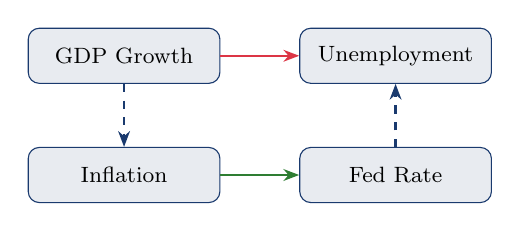
\begin{tikzpicture}[
            node distance=0.5cm,
            box/.style={rectangle, rounded corners, draw=MainBlue, fill=MainBlue!10,
                        text width=2.2cm, minimum height=0.7cm, align=center, font=\footnotesize},
            arrow/.style={-{Stealth[length=2mm]}, thick, MainBlue}
        ]
            \node[box] (gdp) {GDP Growth};
            \node[box, right=1cm of gdp] (unemp) {Unemployment};
            \node[box, below=0.8cm of gdp] (infl) {Inflation};
            \node[box, right=1cm of infl] (fed) {Fed Rate};

            \draw[arrow, IDAred] (gdp) -- (unemp);
            \draw[arrow, Forest] (infl) -- (fed);
            \draw[arrow, dashed] (gdp) -- (infl);
            \draw[arrow, dashed] (fed) -- (unemp);
        \end{tikzpicture}
    \end{center}

    \vspace{0.3em}
    \begin{columns}[T]
        \begin{column}{0.48\textwidth}
            \textbf{Key Findings:}
            \begin{itemize}
                \item GDP Granger-causes unemployment
                \item Inflation Granger-causes Fed policy
                \item VAR captures these dynamics
            \end{itemize}
        \end{column}
        \begin{column}{0.48\textwidth}
            \textbf{Practical Applications:}
            \begin{itemize}
                \item Economic forecasting
                \item Policy analysis
                \item Risk management in portfolios
            \end{itemize}
        \end{column}
    \end{columns}
\end{frame}

%=============================================================================
% SECTION 6: MODEL SELECTION GUIDE
%=============================================================================
\section{Model Selection: A Practical Guide}

\begin{frame}{Decision Framework}
    \begin{center}
        \includegraphics[width=0.90\textwidth, height=0.70\textheight, keepaspectratio]{ch10_model_selection_flowchart.pdf}
    \end{center}
\end{frame}

\begin{frame}{Model Selection Summary}
    \begin{table}[h]
        \footnotesize
        \centering
        \begin{tabular}{p{2.5cm}p{3.5cm}p{3.5cm}p{3cm}}
            \toprule
            \textbf{Data Type} & \textbf{Characteristics} & \textbf{Recommended Model} & \textbf{Alternatives} \\
            \midrule
            Financial returns & No trend, volatility clustering & ARIMA-GARCH & EGARCH, GJR \\
            \addlinespace
            Single seasonality & Trend + one seasonal period & SARIMA & ETS, Prophet \\
            \addlinespace
            Long cycles & Sunspots, business cycles & AR + Fourier, TBATS & Spectral methods \\
            \addlinespace
            Structural breaks & COVID, regime changes & Prophet & Intervention ARIMA \\
            \addlinespace
            Multiple series & Interdependencies & VAR, VECM & Factor models \\
            \bottomrule
        \end{tabular}
    \end{table}
\end{frame}

\begin{frame}{Forecast Evaluation Metrics}
    \begin{columns}[T]
        \begin{column}{0.48\textwidth}
            \textbf{Point Forecast Metrics:}

            \vspace{0.3em}
            \textbf{RMSE} (Root Mean Square Error):
            \[
                \sqrt{\frac{1}{n}\sum_{i=1}^{n}(y_i - \hat{y}_i)^2}
            \]

            \textbf{MAE} (Mean Absolute Error):
            \[
                \frac{1}{n}\sum_{i=1}^{n}|y_i - \hat{y}_i|
            \]

            \textbf{MAPE} (Mean Absolute \% Error):
            \[
                \frac{100}{n}\sum_{i=1}^{n}\left|\frac{y_i - \hat{y}_i}{y_i}\right|
            \]
        \end{column}
        \begin{column}{0.48\textwidth}
            \textbf{When to Use Each:}
            \begin{itemize}
                \item \textbf{RMSE}: Penalizes large errors more
                \item \textbf{MAE}: Robust to outliers
                \item \textbf{MAPE}: Scale-independent
            \end{itemize}

            \vspace{0.5em}
            \begin{alertblock}{Cross-Validation}
                Always use time series CV:
                \begin{itemize}
                    \item Rolling window
                    \item Expanding window
                    \item Never shuffle!
                \end{itemize}
            \end{alertblock}
        \end{column}
    \end{columns}
\end{frame}

%=============================================================================
% SECTION 6: SUMMARY
%=============================================================================
\section{Summary and Key Takeaways}

\begin{frame}{Course Summary: Complete Toolkit}
    \begin{columns}[T]
        \begin{column}{0.48\textwidth}
            \textbf{Understanding the Data}
            \begin{itemize}
                \item Visualization first!
                \item Test for stationarity (ADF, KPSS)
                \item Identify seasonality patterns
                \item Check for structural breaks
            \end{itemize}

            \vspace{0.5em}
            \textbf{Classical Models}
            \begin{itemize}
                \item ARIMA: Non-seasonal data
                \item SARIMA: Single seasonality
                \item GARCH: Volatility modeling
            \end{itemize}
        \end{column}
        \begin{column}{0.48\textwidth}
            \textbf{Modern Approaches}
            \begin{itemize}
                \item Prophet: Interpretable, handles breaks
                \item TBATS: Multiple/long seasonalities
                \item VAR/VECM: Multiple time series
            \end{itemize}

            \vspace{0.5em}
            \textbf{Best Practices}
            \begin{itemize}
                \item Always check diagnostics
                \item Use cross-validation
                \item Compare multiple models
                \item Domain knowledge matters!
            \end{itemize}
        \end{column}
    \end{columns}
\end{frame}

\begin{frame}{Final Recommendations}
    \begin{enumerate}
        \item \textbf{Start Simple}: Begin with visualization and basic statistics
        \item \textbf{Test Assumptions}: Stationarity, normality, independence
        \item \textbf{Iterate}: Model $\rightarrow$ Diagnose $\rightarrow$ Improve
        \item \textbf{Compare}: Never rely on a single model
        \item \textbf{Validate}: Out-of-sample testing is essential
        \item \textbf{Communicate}: Clear visualizations and interpretations
    \end{enumerate}

    \vspace{0.5em}
    \begin{exampleblock}{Remember}
        ``All models are wrong, but some are useful.'' --- George Box

        \vspace{0.3em}
        The goal is not perfect prediction, but useful insights and reasonable forecasts.
    \end{exampleblock}
\end{frame}

\begin{frame}{Questions?}
    \begin{center}
        \Large\textcolor{MainBlue}{Questions?}

        \vspace{1cm}

        \normalsize
        \textbf{Next Steps:}
        \begin{itemize}
            \item Practice with the Jupyter notebook
            \item Apply these methods to your own data
            \item Compare different models on the same dataset
        \end{itemize}

        \vspace{0.5cm}

        Course Materials: \texttt{github.com/danpele/Time-Series-Analysis}
    \end{center}
\end{frame}

\end{document}
